\subsubsection{Methodology BI-LSTM}

For the model based on the BI-LSTM architecture, the full embeddings generated by the roBERTa model were used, and the architecture shown in Figure~\ref{fig:bilstm_architecture}, as recommended in \cite{fieri2023offensive}, was implemented. This architecture was trained using the Adam optimizer for 200 epochs, storing the checkpoint that achieved the highest accuracy on the validation set. This validation set accounted for 15\% of the data, as did the test set, while the remaining 70\% was used for training. 

After training, the best checkpoint was restored and performance evaluation was carried out. The model was assessed using the same metrics as with the XGBoostClassifier: precision, recall, F1-score, accuracy, and the confusion matrix.

\begin{figure}[htbp]
  \centering
  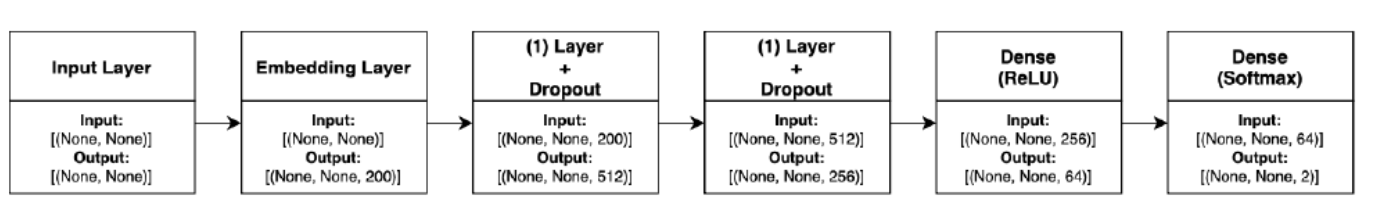
\includegraphics[width=0.45\textwidth]{images/bilstm_architecture.png}
  \caption{BI-LSTM architecture used in the model.}
  \label{fig:bilstm_architecture}
\end{figure}